\section{Implementation}
\label{sec:impl}
\begin{figure}[t]
  \centering
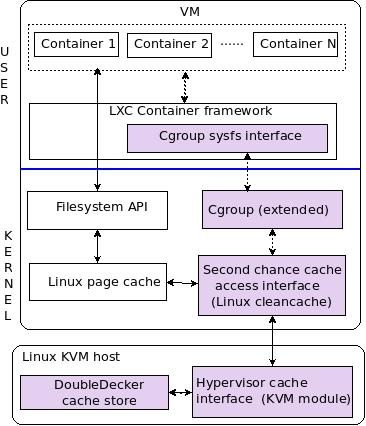
\includegraphics[width=0.4\textwidth]{images/implementation} 
 \caption{\dd{} implementation in KVM virtualized system. The shaded 
 boxes in the figure represents modified/enhanced software components.
% \puru{this figure not refered in text?}
}%
 \vspace{-0.5cm}
 \label{fig:impl} 
\end{figure}

We implemented the \dd{} solution on the Linux+KVM virtualization
platform and LXC~\cite{lxc} containers.
%We have implemented \dd{} in Linux KVM hypervisor platform.
%
Guest OS modifications are implemented in Linux virtual machines
hosting LXC~\cite{lxc} containers.
%
Linux \texttt{cleancache}, the second chance cache access interface 
is modified to implement the \cgroup{} extensions required for \dd{} (Figure~\ref{fig:impl}).
%hypervisor cache store.
%
Linux \cleancache{} operations are routed to the KVM hypervisor through 
a new VMCALL~\cite{intelmanual}.
%
As shown in Figure~\ref{fig:impl}, the KVM hypervisor module is 
modified to capture this hypercall, 
copy the arguments on to the host memory and pass the call to 
the \dd{} hypervisor cache store. 
 

\subsection{\cgroup{} and \cleancache{} modifications}
%
Several modifications to the Linux \cgroups{} subsystem
are required for container-level nested hypervisor cache management.
%
Two new parameters have been added to the kernel
state description of the \cgroups{} subsystem---
(i) name of the \cgroups{} for
which the hypervisor cache is to be enabled, 
(ii) policy configuration tuple ($<$\texttt{T, W}$>$) for each container 
to specify 
the storage type and weight percentage.
%\puru{what is identification filter?.}
%
These parameters can be accessed as \texttt{sysfs} entries 
from the user space.
%user space 
%(sysfs) configurations---(i) name or identification filter of the \cgroups{} for
%which the hypervisor cache is to be enabled, (ii) policy configuration tuple
%for each container to specify the storage type and weightage percentage.
%
Interactions between the \cgroup{} subsystem and the \cleancache{} interface
occur only if the \cgroup{} identifier matches the provided filter.
%
The newly introduced second chance operations and the events triggering these 
are described below.
%

\vspace{0.15cm}
\noindent
{\bf CREATE\_CGROUP:} When a new container is created, a new \cgroup{}
kernel state is created and
the \cleancache{} interface is notified of the event.
%
Linux \cleancache{} is extended to handle a container creation event and 
which in turn forwards this event to the \dd{} hypervisor cache store.
%
The \dd{} cache returns a new unique pool identifier (\texttt{pool-id}) 
corresponding to the newly created container. 
%
The pool-id is stored
in the \cgroup{} kernel state of the guest OS and used for subsequent
hypervisor cache operations.
%which
%is stored in the kernel \cgroup{} state corresponding to the container and used in
%subsequent hypervisor cache operations. 
%

\vspace{0.15cm}
\noindent
{\bf SET\_CG\_WEIGHT:} 
%The administrator changes the weight configurations---storage type or
%weightage percentage---for a container through the \cgroup{} sysfs user space interface.
%
This event is generated when the \cgroup{} sysfs entry is updated 
(due to policy control decision) to update the container hypervisor
cache specifications---the storage type and weight percentage.
%\puru{need to make consistent---weight vs. ratios.}
%
Update to the \cgroup{} variables is captured by Linux 
kernel \cgroup{} module and passed on to the \cleancache{} layer. 
%
The \cleancache{} second chance cache interface transmits the specifications
to the \dd{} hypervisor cache manager via KVM hypercall. 
%\puru{verify this}.
The \dd{} cache manager updates its state for the container
and updates state of the cache as necessary.
%to reflect the configuration changes in the hypervisor cache store.
%
 
\vspace{0.15cm}
\noindent
{\bf MIGRATE\_OBJECT:} 
Since the \emph{key} used by hypervisor cache to index objects
is \cgroup{} based and not based on file system information,
a subtle issue arises due to mapping of files to
application containers.
%Due to the transition from file system level key generation to 
%\cgroups, there could be subtle issues regarding mapping the file blocks to the application
%container.
%
Specifically, this is the case when \cgroup{} ownership for file 
blocks present in the hypervisor cache store changes from one \cgroup{} 
to another. 
%
This is usually the case when files are shared
across application containers.
%
%This can happen when some files are shared across application containers.
%
To handle this condition, file blocks are migrated (mappings changed)
from one hypervisor cache pool (corresponding to a container) to another.
%

\vspace{0.15cm}
\noindent
{\bf DESTROY\_CGROUP:} When a container with a valid \texttt{pool-id} is shutdown, 
the \cleancache{} interface is notified of the event.
%
Linux \cleancache{} is extended to handle a container destroy event and 
%is pass on
transmits the event to the \dd{} cache manager.
%
The hypervisor cache frees up all the objects corresponding to the pool 
and marks the pool as free.


\vspace{0.15cm}
\noindent
{\bf GET\_STATS:} It can be useful for the policy controller inside a VM to 
get per-container level cache allocation and cache usage related statistics  
for the containers executing in the VM.
%
We have extended the \cleancache{} interface to request the \dd{} cache
for statistics when required by the policy controller.
 

With \dd, semantics of existing \cleancache{} operations---lookup (\get), 
store (\put), invalidate (\flush)
(refer \S\ref{sec:bg}) remain the same, their implementation 
has the following modifications.
%
The page cache layer passes a memory page along with the
file inode number and block offset to the \cleancache{} layer to 
enable second chance operations.
%
With vanilla \cleancache{} implementation, there is one-to-one 
correspondence between the \texttt{pool-id} and the file system 
superblock which can be extracted easily during \cleancache{} operations.
%to carry out the above operations.
%
With \dd{}, the \cgroup{} owner is first deduced from the memory 
page to determine the unique \texttt{pool-id}.  
%
This is determined by finding the owner process for the page, 
and extracting the Cgroup entity to which the process belongs.
%\puru{add another line here. page to process to cgroup}.


\subsection{\dd{} hypervisor cache store}
\begin{figure}[t]
  \centering
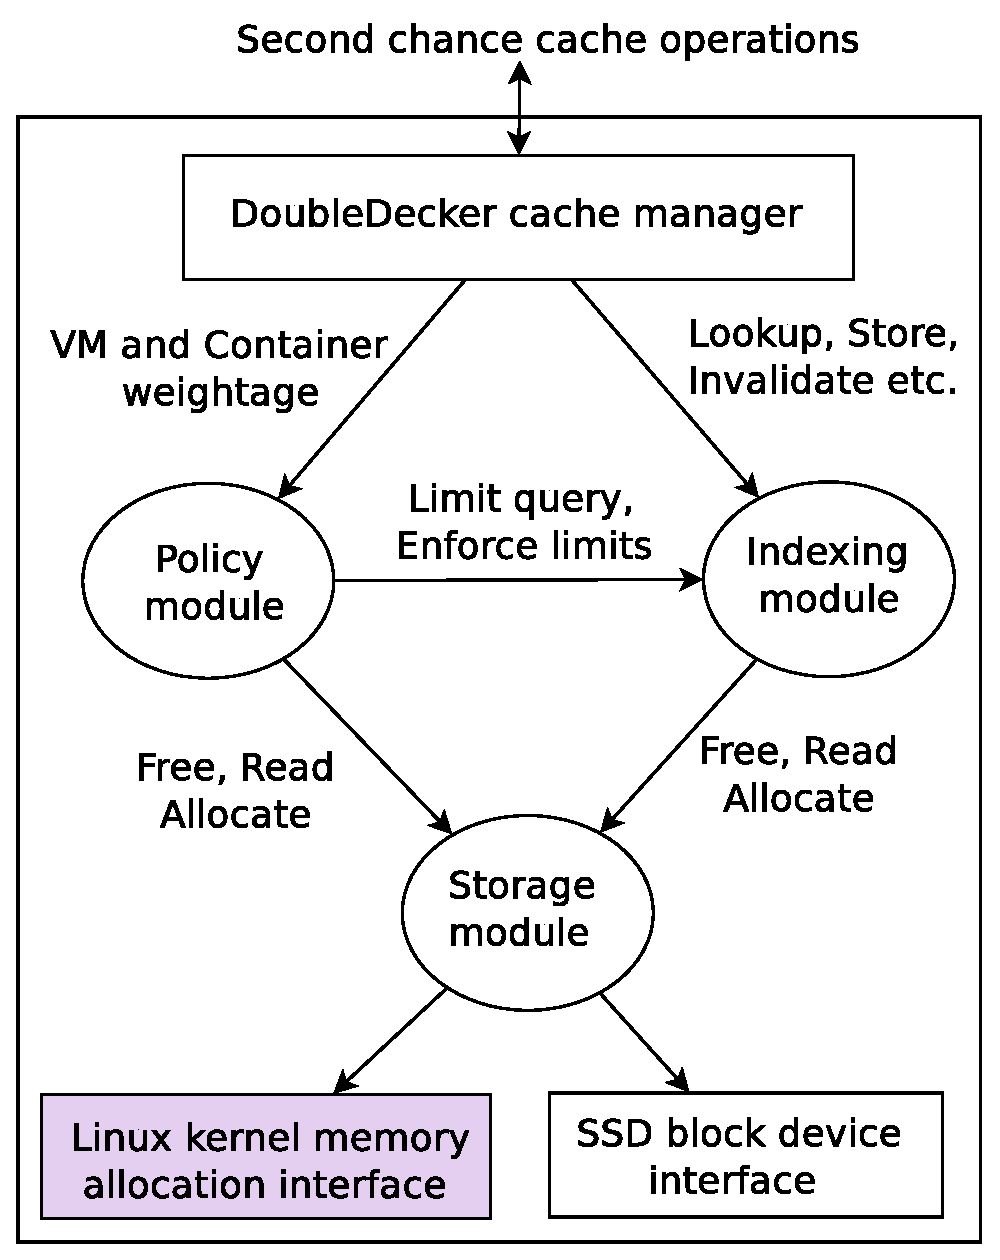
\includegraphics[width=0.33\textwidth]{images/ddecker} 
 \caption{\dd{} hypervisor cache components. 
% \puru{too many bidirectional arrows. Also naming
% consistency is required.}}
  }%
 \vspace{-0.5cm} 
 \label{fig:cachestore} 
\end{figure}
%
High-level design of \dd{} hypervisor cache store implementation 
is shown in Figure~\ref{fig:cachestore}.
%
The \dd{} cache manager interface is the entry point for all 
calls from the guest VMs (routed through the KVM hypervisor
cache interface) and configuration changes by the host administrator.
%\puru{cache access interface vs. hypervisor cache manager. i have
%used the latter a few times earlier.}
%

The host administrator may configure the memory size limits and SSD device 
limits for the \dd{} cache store which is handled by the
policy module.
%
Further, container level configurations explained before is
delegated to the policy module for cache management. 
%
On any configuration change, the policy module recalculates cache store
entitlements at two levels---per-VM level and container (pool) level.
%
The policy module monitors \dd{} cache usage by the VMs and containers and
takes appropriate action (e.g., eviction) when the cache entitlement is
violated.
%
In the current implementation, FIFO is used (LRU equivalent for exclusive caches)
to implement eviction at a pool level.
%
%\revised{
As part of future work, we plan to evaluate different eviction policies
(similar to ExTmem~\cite{extmem}) and provide a knob for 
the VM-level policy controller to employ application specific eviction
policies if desired.
%}
 
%

The indexing module is responsible for implementing normal second chance 
cache operations like lookup (\get), store (\put) etc..
% 
The key consisting of three tuples provided by the VM 
($<$\texttt{pool-id}{}$>$, $<$\texttt{inode-num}{}$>$, $<$\texttt{block-offset}{}$>$)
along with VM ID is used to map the request to storage objects.
%
A hierarchy of indexing data structures---per-pool file object (\texttt{inode-num}) hash 
table, file block radix-tree etc.---are used to map the key to a storage
object.
%
The opaque storage object is exchanged with the storage module
for actual storage operations.   
%
On a \put{} request, the indexing module enforces the limits by
checking the pool entitlement and evicting through the policy module,
if necessary.


Storage module provides backend independent services to 
read storage blocks, allocate new storage blocks and free storage blocks.
%
In the current \dd{} implementation, two types of storage backends are
implemented.
%
For memory storage backend, Linux kernel routines like \texttt{page\_alloc},
\texttt{page\_free}, \texttt{memcpy} etc. are used.
%
For SSD backend implementation, we have implemented a raw block device 
IO layer on top of the generic block device driver interface. 
%
The read calls (for \get{} operations) implements synchronous IO
operations while write calls (for \put{} operations) are implemented in an
asynchronous manner.

\subsection{\dd{} policy enforcement}

\begin{algorithm}[t]
  \caption{Victim selection from a list of cache using entities (VMs or Containers)}\label{algo:evict}
  \begin{algorithmic}[1]
    \Procedure{getvictim}{$Entities[1..n], EvictionSize$}\newline
      \Comment{\textit{EvictionSize}: \# of cached blocks to be evicted}\newline
      \Comment{\textit{Entities}: List of entities (VMs or containers)}
      \State \textit{overusedlist[1..n]}
      \State \textit{cumlweight} = 0
      \State \textit{underusedbuf} = 0
      \State \textit{count} = 0
      \For{i=1 to n}
          \State \textit{E$_i$} = \textit{Entities[i]}
          \If {\textit{E$_i$.entitlement} $<$ \textit{E$_i$.used + EvictionSize}} 
                 \State \textit{overusedlist[count]} = \textit{E$_i$}
                 \State \textit{cumlweight} += \textit{E$_i$.weight}
                 \State \textit{count++}
          \EndIf
          \If {\textit{E$_i$.entitlement}-\textit{E$_i$.used}$>$2$*$\textit{EvictionSize}}
                 \State \textit{underusedbuf} += \textit{E$_i$.entitlement} - \textit{E$_i$.used} 
          \EndIf
      \EndFor
     \State \textit{E} = \textit{overusedlist[1]}
     \State \textit{exceedmax} = exceed(\textit{E}, \textit{underusedbuf}, \textit{cumlweight})
     \For{i=2 to count}
        \State \textit{E$_i$} = \textit{overusedlist[i]}
        \If {\textit{exceedmax} $<$ exceed(\textit{E})}
                    \State \textit{E} = \textit{E$_i$}
                    \State \textit{exceedmax} = exceed(\textit{E})
        \EndIf
     \EndFor
    \State Return E
    \EndProcedure
  \end{algorithmic}
  \label{algo:victim}
\end{algorithm}

%
To implement resource conservative cache management,
cached blocks are evicted only when the \dd{} cache limit is reached.
%
In such a case, selecting a victim application (container) is a two step process---first victim
VM is selected and then the victim container in the selected VM is 
decided.
%
Victim selection algorithm is same for both the levels (VMs and containers) and outline of 
the algorithm is presented in Algorithm~\ref{algo:victim}.
% 
The algorithm takes list of entities (VMs or Containers) and eviction size 
as input to return the victim entity.
%
List of entities who are over the limit of their entitlement---calculated directly
applying the \dd{} cache weight configuration---are determined (line\# 8-12) and
stored in the \textit{overusedlist}.  
%
Sum of underutilized memory (\textit{underusedbuf}) is redistributed among
the entities as per their weights to calculate their effective entitlements 
(\textit{E.entitlement} + (\textit{b} * \textit{E.weight} / \textit{cw}))
and exceed values.
%
The exceed value for an entity is calculated as,
\begin{equation}
\begin{aligned}
exceed(\textit{E}, \textit{b}, \textit{cw}) = \textit{E.used} + \textit{EvictionSize} - \\
                                              (\textit{E.entitlement} + (\textit{b} * \textit{E.weight} / \textit{cw}))
\end{aligned}
\end{equation}
where \textit{b} is the sum of under utilized entitlements (\textit{underusedbuf} in
Algorithm~\ref{algo:evict}), \textit{cw} is the sum of weight percentages of entities whose cache
usage is above their respective entitlements.
%
The entity calculated with the highest exceed value is selected as the 
victim for eviction.
%
Only one victim entity is selected because 
we use a small batch (2MB) for eviction when a store request can not be
serviced because of global limit violations.
